% -*-coding: latin-9;-*-

% Not all the slides here are shown, but keep them for other presentations
\let\ifPresentHiddenSlides=\iffalse

% For Ubuntu 22.04, it looks like the
% xcolor={dvipsname,svgnames,x11names} is not enough to have color
% Coral
\PassOptionsToPackage{dvipsname,svgnames,x11names}{xcolor}


%% To deal with the colors and number of slides per page according to the
%% \VersionPapier switch :
\ifx\VersionExpose\UnTrucInexistant%

% The handout version
\documentclass[aspectratio=169,handout,compress,10pt,hyperref={hyperindex},xcolor={dvipsname,svgnames,x11names}]{beamer}
\usepackage{pgfpages}
\pgfpagesuselayout{4 on 1}[a4paper,landscape,border shrink=5mm]
\else
% The slide version
\documentclass[aspectratio=169,compress,10pt,hyperref={hyperindex},xcolor={dvipsname,svgnames,x11names}]{beamer}
\fi

\usepackage[latin9]{inputenc}

\usepackage{header_SYCL}

% Some specialization according to the official AMD 2022 PowerPoint
% template
\usepackage{beamer_AMD_2022}

% To add arrows between slide pieces:
% Here because of catcode wizardy I guess :-(
% Should go into tikz_hpc
% Could use \pgftext instead of using "text depth=0pt"
\newcommand{\PlaceTextNode}[2]{\tikz{\node[inner sep=0pt,text depth=0pt] (#1) {#2};}}

% To decorate some lstlisting lines:
\usepackage{balloon_rk}

% Use SYCL+OpenCL as the default language
\lstset{language=SYCL,showstringspaces=false,
  basicstyle=\small}

%\tracingall

\author[]{Ronan Keryell (\url{ronan.keryell@amd.com})}

\title{C++ and Khronos computing standards}

\subtitle{OpenCL, SYCL (and Vulkan, OpenVX?)}

\date{2023/06/06 @ Khronos OpenCL WG}

\institute[\copyright{} Copyright 2023 Khronos]{Fellow Software
  Development Engineer @ AMD Research \& Advanced Development\\
  % San Jos�, California\\
  Khronos SYCL specification editor \& ISO C++ committee member}

% Remove the logo
%%\pgfdeclareimage[width=0.8cm]{logo-SYCL}{Khronos/Logos/SYCL/SYCL_500px_June16}
%%\logo{\hbox to 0.75cm{\vbox{%
%%      \href{https://www.khronos.org/sycl}{\pgfuseimage{logo-SYCL}}}}}
\logo{}

\begin{document}

\SetImageBackground{Background/Khronos-background-16-9}
{
  %\SetImageBackground{Background/AMD/Corporate_Template/Presentations_Templafy/Corporate_PPT_Template-White_Background-6x9-title_page-23.pdf}

  \begin{frame}[plain]
%\tracingall=1
    \titlepage
%\tracingall=0
  \end{frame}
}

\begin{frame}{Remember C++ ?}
  \begin{BoiteA}{2-line description by Bjarne Stroustrup}
    \begin{itemize}
    \item Direct mapping to hardware
    \item Zero-overhead abstraction
    \end{itemize}
  \end{BoiteA}
\end{frame}


\begin{frame}[fragile]{Modern Python/C/Modern C++/Old C++}
  \begin{multicols}{2}
    \begin{itemize}
    \item Python 3.11
      \begin{lstlisting}[language=Python]
v = [ 1, 2, 3, 5, 7 ]
print(v)
      \end{lstlisting}
      \url{https://godbolt.org/z/Kq9vc1jhY}
    \item C99 (also usable in C++)
      \begin{lstlisting}
#include <stdio.h>
int a[] = { 1, 2, 3, 5, 7 };
for (int i = 0;
     i < sizeof(a)/sizeof(a[0]);
     ++i)
  printf("%d ", a[i]);
      \end{lstlisting}

      \columnbreak

    \item C++23
      \begin{lstlisting}
import std;
std::vector v { 1, 2, 3, 5, 7 };
std::println("{}", v);
      \end{lstlisting}
    \item C++03
      \begin{lstlisting}
#include <iostream>
#include <vector>
std::vector<int> v;
v.push_back(1);
v.push_back(2);
v.push_back(3);
v.push_back(5);
v.push_back(7);
for (std::vector<int>::iterator i =
       v.begin(); i != v.end(); ++i)
  std::cout << *i << std::endl;
      \end{lstlisting}
    \end{itemize}
  \end{multicols}
\end{frame}


\begin{frame}
  \Huge
  \begin{center}
    But...\\
    No heterogeneous computing in C++\\
    \frownie
  \end{center}
\end{frame}


\SlideFromImageFile{About_Khronos_Slide-2018}


\begin{frame}{OpenCL and C++}
  Non-single source API
  \begin{itemize}
  \item Host C API to control the device with various C++ wrappers and
    other languages
    \begin{itemize}
    \item Old Khronos C++ wrapper v1 (C++03)
    \item Less old Khronos C++ wrapper v2 (C++11)
      \url{https://github.khronos.org/OpenCL-CLHPP}
      \url{https://github.com/KhronosGroup/OpenCL-Headers}
    \item Boost.Compute {https://github.com/boostorg/compute}
    \item + everybody developing own C++ (or other languages) wrappers
    \end{itemize}
  \item Kernel source code or binary (SPIR or target)
    \begin{itemize}
    \item Legacy OpenCL C source code
    \item OpenCL C++ 1.0 for OpenCL 2.2
      \begin{itemize}
      \item Inspired by SYCL 2.2 modernism but incompatible with
        legacy OpenCL C
      \end{itemize}
    \item Khronos-friendly-but-independent \emph{C++ for OpenCL} in
      Clang/LLVM \url{https://clang.llvm.org/docs/OpenCLSupport.html}
      \url{https://www.khronos.org/opencl/assets/CXX_for_OpenCL.html}
    \end{itemize}
  \item Split-source + JIT allows easy meta-programming with strings
  \end{itemize}
\end{frame}



\begin{frame}{SYCL ecosystem is growing}
  \centerline{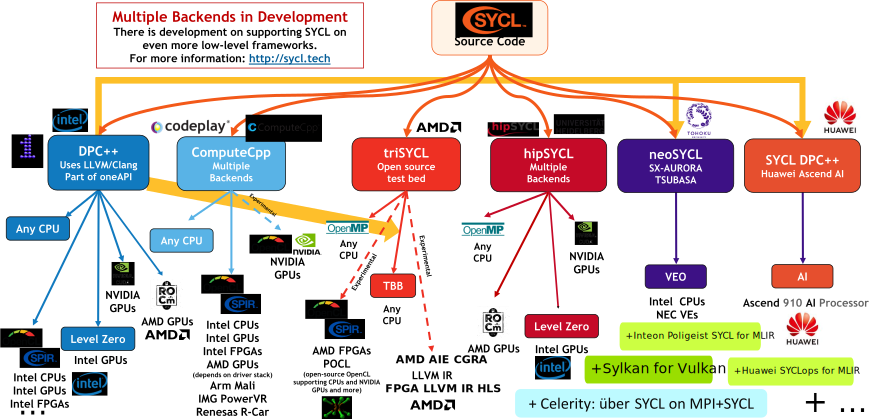
\includegraphics[height=0.8\textheight]{Images/Languages/SYCL/Implementations/SYCL-ecosystem-2023-04-13}}
  \url{https://www.khronos.org/blog/sycl-2020-what-do-you-need-to-know}
\end{frame}


\begin{frame}[fragile]{SYCL 2020 $\equiv$ heterogeneous simplicity with modern C++}
  % Add the descriptive boxes
  \begin{tikzpicture}[remember picture, overlay]
    \scriptsize
    \node<2-> [
      xshift=-0.3\paperwidth,
      yshift=-0.1\paperheight,
      anchor=north east
    ](bufferNode)
    at (current page.north east)
    {
      \scriptsize
      \begin{BoiteA}[width=0.33\hsize]{Abstract storage}
        \begin{itemize}
        \item Host or device (remote) memory
        \end{itemize}
      \end{BoiteA}
    };

    \node<3-> [
      %xshift=-0.1\paperwidth,
      yshift=-0.25\paperheight,
      anchor=north east
    ](kernelNode)
    at (current page.north east)
    {
      \scriptsize
      \begin{BoiteA}[width=0.33\hsize]{Code executed on device (``kernel'')}
        \begin{itemize}
        \item ``Single-source''
        \item Seamless integration in host code
        \item Type-safety
        \item Asynchronous execution
        \end{itemize}
      \end{BoiteA}
    };

    \node<4-> [
      %xshift=0.25\paperwidth,
      yshift=0.05\paperheight,
      anchor=south east
    ](accessorNode)
    at (current page.south east)
    {
      \scriptsize

      \begin{BoiteA}[width=0.38\hsize]{Accessor}
        \begin{itemize}
        \item Express access intention
        \item Implicit data flow graph
        \item Automatic data transfers across devices
        \item Overlap computation \& communication
        \end{itemize}
      \end{BoiteA}
    };
    \node<5-> [
      xshift=-0.05\paperwidth,
      yshift=-0.1\paperheight,
      anchor=north west
    ](queueNode)
    at (current page.north west)
    {
      \scriptsize

      \begin{BoiteA}[width=0.32\hsize]{Queue}
        \begin{itemize}
        \item Direct work to specific accelerator
        \item Submission of a command group
        \end{itemize}
      \end{BoiteA}
    };
    % Add arrows from boxes too source code
    \draw<2-> [overlay,->,very thick,red] (node cs:name=bufferNode) to (pic cs:buffer);
    \draw<3-> [overlay,->,very thick,red] (node cs:name=kernelNode) to (pic
      cs:kernel);
    \draw<3-> [overlay,-,line width=6mm,yellow] (pic cs:kernelStart) to (pic cs:kernel);
    \draw<4-> [overlay,->,very thick,red] (node cs:name=accessorNode) to (pic cs:accessor);
    \draw<4-> [overlay,->,very thick,red] (node cs:name=accessorNode) to (pic cs:hostAccessor);
    \draw<5-> [overlay,->,very thick,red] (node cs:name=queueNode) to (pic cs:queue);
  \end{tikzpicture}
  \begin{lstlisting}[name=SYCLsample]
#include <iostream>
#include <sycl/sycl.hpp>
constexpr int n = 32;

int main () {
  sycl::buffer<int> buf�\tikzmark{buffer}� { n };
  sycl::�\tikzmark{queue}�queue {}.submit([&](auto &h) {
      sycl::accessor a { buf, h, sycl::write_only, sycl::no_init }�\tikzmark{accessor}�;
      h.parallel_for(n, �\tikzmark{kernelStart}�[=](auto i) { a[i] = i; }�\tikzmark{kernel}�);
  });
  for (sycl::host_accessor a { buf }�\tikzmark{hostAccessor}�; auto e : a)
      std::cout << e << std::end;
}
  \end{lstlisting}
\end{frame}


\begin{frame}{Some of the existing SYCL back-ends}
  \centerline{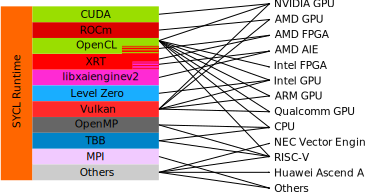
\includegraphics[height=0.8\textheight]{Images/Languages/SYCL/Implementations/sycl_rt_backend_hardware}}
\end{frame}


\begin{frame}{Unique SYCL feature: interoperability with backends}
  \begin{itemize}
  \item Porting existing code
    \begin{itemize}
    \item Code already based on OpenCL/CUDA/OpenMP/HIP/\ldots{} (or
      whatever backend)
    \item Want to change just part of application to use SYCL
    \end{itemize}
  \item Incorporating a backend module into a SYCL application
    \begin{itemize}
    \item Application based on SYCL
    \item Want to call some OpenCL/CUDA/OpenMP/HIP/\ldots{} library
      (or whatever backend)
    \end{itemize}
  \item Take advantage of backend-specific features
  \item Disadvantage: reduces portability!
    \begin{itemize}
    \item Not all implementations may support your backend
    \end{itemize}
  \item[\vavers] Unique feature of SYCL!
  \end{itemize}

  {\scriptsize
    %% IWOCL and SYCLcon 2022
    %% Using Interoperability Mode in SYCL 2020
    Aksel ALPAY, Thomas APPLENCOURT, Gordon BROWN, Ronan KERYELL and
    Gregory LUECK. ``Using interoperability mode in SYCL 2020.'' In
    SYCLcon 2022: International Workshop on SYCL. Association for
    Computing Machinery, May 2022. doi:10.1145/3529538.3529997.
    \url{https://www.iwocl.org/wp-content/uploads/39-presentation-iwocl-syclcon-2022-aksel.pdf}
    \url{https://www.youtube.com/watch?v=XIPhuesdqYE}
  }
\end{frame}


\begin{frame}[fragile]{Type 1: SYCL object from backend object}
  \framesubtitle{``Higher-level XRT'' for AMD FPGA in 43 lines with SYCL}
  \begin{multicols}{2}
    \begin{lstlisting}[basicstyle=\tiny]
#include <cassert>
#include <sycl/sycl.hpp>
#include <sycl/ext/xilinx/xrt.hpp>
#include <xrt.h>
#include <xrt/xrt_kernel.h>
constexpr int size = 4;
int main() {
  sycl::buffer<int> a { size };
  sycl::buffer<int> b { size };
  sycl::buffer<int> c { size };
  {
    sycl::host_accessor a_a { a };
    sycl::host_accessor a_b { b };
    for (int i = 0; i < size; ++i) {
      a_a[i] = i;
      a_b[i] = i + 42;
    }
  }
  sycl::queue q;
  xrt::device xdev =
    sycl::get_native<sycl::backend::xrt>(q.get_device());
  xrt::kernel xk { xdev, xdev.load_xclbin("vadd.hw_emu.xclbin"),
                   "vadd" };
  sycl::kernel k
    { sycl::make_kernel<sycl::backend::xrt>(xk, q.get_context()) };

  q.submit([&](sycl::handler& cgh) {
    cgh.set_args(sycl::accessor { a, cgh, sycl::read_only },
                 sycl::accessor { b, cgh, sycl::read_only },
                 sycl::accessor { c, cgh, sycl::write_only,
                                  sycl::no_init },
                 size);
    cgh.single_task(k);
  });
  {
    sycl::host_accessor a_a { a };
    sycl::host_accessor a_b { b };
    sycl::host_accessor a_c { c };
    for (int i = 0; i < size; ++i) {
      int res = a_a[i] + a_b[i];
      int val = a_c[i];
      assert(val == res);
    }
  }
}
    \end{lstlisting}
  \end{multicols}
  {\tiny\url{https://github.com/keryell/heterogeneous_examples/blob/main/vector_add/SYCL/vector_add_XRT_interoperability.cpp}}

  \begin{BoiteA}{Typical usage}
    Adding SYCL functionality to an existing backend-specific application
  \end{BoiteA}
\end{frame}

\begin{frame}[fragile]{Type 2: backend object from SYCL object}
  \begin{lstlisting}
void MyFunc(sycl::device dev) {
#ifdef SYCL_BACKEND_OPENCL
  cl_device_id clDev = sycl::get_native<sycl::backend::opencl>(dev);

  char builtins[SIZE];
  size_t sz;
  clGetDeviceInfo(clDev, CL_DEVICE_BUILT_IN_KERNELS, SIZE, builtins, &sz);
  /* Use OpenCL builtin kernel...*/
#else
  /* fallback if no OpenCL backend */
#endif
}
  \end{lstlisting}

  \begin{BoiteA}{Typical usage}
    Incorporate a backend-specific library into a SYCL application or
    take advantage of a backend-specific feature
  \end{BoiteA}
\end{frame}

\begin{frame}[fragile]{Type 3: schedule a backend-specific command}
  \begin{lstlisting}
void MyFunc(sycl::queue q, sycl::buffer<int> buf) {
#ifdef SYCL_BACKEND_OPENCL
  q.submit([&](sycl::handler &cgh) {
    sycl::accessor acc{buf, cgh};
    cgh.host_task([=](sycl::interop_handle &ih) {
      cl_mem clMem = ih.get_native_mem<sycl::backend::opencl>(acc)[0];
      /* use OpenCL APIs with clMem */
    });
  });
#endif
}
  \end{lstlisting}
  \begin{BoiteA}{Typical usage}
    Incorporate a backend-specific library or feature into a SYCL task graph
  \end{BoiteA}
\end{frame}



\begin{frame}{Culture}
  \begin{itemize}
  \item No real C++ culture inside OpenCL WG
    \begin{itemize}
    \item Designing a C++ API requires some cultural knowledge
    \item Several vendor implementations are forks from initial Apple
      contribution
      \begin{itemize}
      \item Do not benefit from open-source goodies
      \item Huge technical debt, no portable IR,\ldots
      \item Require other producers to rely on LLVM IR or MLIR to
        OpenCL C backend
      \end{itemize}
    \end{itemize}
  \item SYCL is all about C++
    \begin{itemize}
    \item Need to be close to Clang/LLVM upstream
      \begin{itemize}
      \item Otherwise painful technical debt management
      \end{itemize}
    \end{itemize}
  \item Vulkan has some C++ culture in the host API
  \end{itemize}
\end{frame}

\begin{frame}[fragile]{Conclusion}
  \begin{itemize}
  \item Do we care?
  \item Who wants to push C++?
  \item Cultural? Market? Politics? Religious?
  \item C++ and API: large design space, depend on C++ version...
  \item Provide directions to programmers interested by C++
    to pick an API?
  \item Just split-source vs single-source independent from C++ aspects?
  \end{itemize}
\end{frame}


\section*{Table of content}

\begin{multicols}{2}
  \tiny
  \tableofcontents[frametitles]
  \textbf{You are here      !}\hfill\expandafter\the\csname c@page\endcsname
\end{multicols}


\end{document}


%%% Local Variables:
%%% mode: latex
%%% ispell-local-dictionary: "american"
%%% TeX-auto-untabify: t
%%% TeX-PDF-mode: t
%%% TeX-master: t
%%% End:
% vim:spell spelllang=en
